\documentclass[a4paper,12pt]{article}

% pobranie bibliotek

\usepackage[T1]{fontenc}    % pobranie bibliotek
\usepackage[utf8]{inputenc}
\usepackage[polish]{babel}
\usepackage{graphicx}
\usepackage{booktabs}
\usepackage{amsmath}
\usepackage{amsfonts}
\usepackage{amssymb}
\usepackage{etexcmds}
\usepackage{hyperref}
\usepackage{float}

\graphicspath{{images/}} 



% METADATA
\newcommand{\authorName}{Filip Mitura  \\ grupa 3, Numer Indeksu: 312153 \ \\Hubert Mizura \ \\grupa 2, Numer indeksu 312155}
\newcommand{\titeReport}{Projekt nr 3 \\ Wtyczka do programu QGIS - PyQGIS}
\newcommand{\titleLecture}{Informatyka geodezyjna 2 \\ sem. IV, ćwiczenia, rok akad. 2022-2023} 
\newcommand{\kind}{report}
\newcommand{\supervisor}{....}
\newcommand{\gikweb}{\href{www.gik.pw.edu.pl}{www.gik.pw.edu.pl}}
\newcommand{\institut}{Zakład Geodezji Wyższej i Astronomii}
\newcommand{\faculty}{Wydział Geodezji i Kartografii}
\newcommand{\university}{Politechnika Warszawska}
\newcommand{\city}{Warszawa}
\newcommand{\thisyear}{2022}
%\date{}
% PDF METADATA
\pdfinfo
{
	/Title       (GIK PW)
	/Creator     (TeX)
	/Author      (Imię Nazwisko)
}


% ------------------------- POCZATEK DOKUMENTU -------------------
\begin{document}
	\begin{figure}
		\centering
		
\includegraphics[width=0.7\textwidth]{gik.png}
	\end{figure}
	\begin{center} 
		\rule{\textwidth}{.5pt} \\
		\vspace{1.0cm}
		\Large \textsc{\titeReport}
		\vspace{0.5cm} \\  
		\large \textsc{\titleLecture}
		\vspace{0.5cm}\\
		\textsc{\authorName}  \\
		
		\textsc{\faculty}, \textsc{\university}  \\ 
		\city, \today
	\end{center} 
	\rule{\textwidth}{0.5pt}
	
	\newpage
	\section{Opis projektu}
	Projekt polegał na stworzeniu funkcjonalnej wtyczki do wykonywania obliczeń a także przedstawiania informacji takich jak nazwa wybranej warstwy lub ilość zaznaczanych punktów. Proces tworzenia wtyczki składał się z utworzenia samej wtyczki, które polegało na wybraniu odpowiednich ustawień, nazw oraz jej opisu. Nastęnie należało zaprojektować część graficzną interfejsu w QtDesignerze, dokonać konwersji pliku .ui do .py oraz stworzyć mechnizm obsługi zdarzeń widgetów, czyli powiązanie odpowiednich funkcji, algorytmów ze zmianami następującymi w części graficznej. Mechanizm slotów oraz sygnałów stanowił najważniejszy element projektu, ponieważ bez niego wtyczka nie byłaby funkcjonalna.\newline
	
	\section{Obsługa wtyczki}
	\subsection{Uruchomienie wtyczki}
	Algorytm wymienionych wyżej obliczeń znajduje się w pliku $"wtyczka\_projekt\_dialog.py"$. W celu uruchomienia wtyczki należy otworzyć program $"QGIS"$. Następnie jeśli wtyczka została zainstalowana uruchamiamy ją poprzez odpowiednią ikonę:
	\begin{figure}[H]
		\centering
		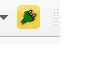
\includegraphics[width=0.3\textwidth]{w.png}
	\end{figure}
 Powinno otworzyć się poniższe okno:
	\begin{figure}[H]
		\centering
		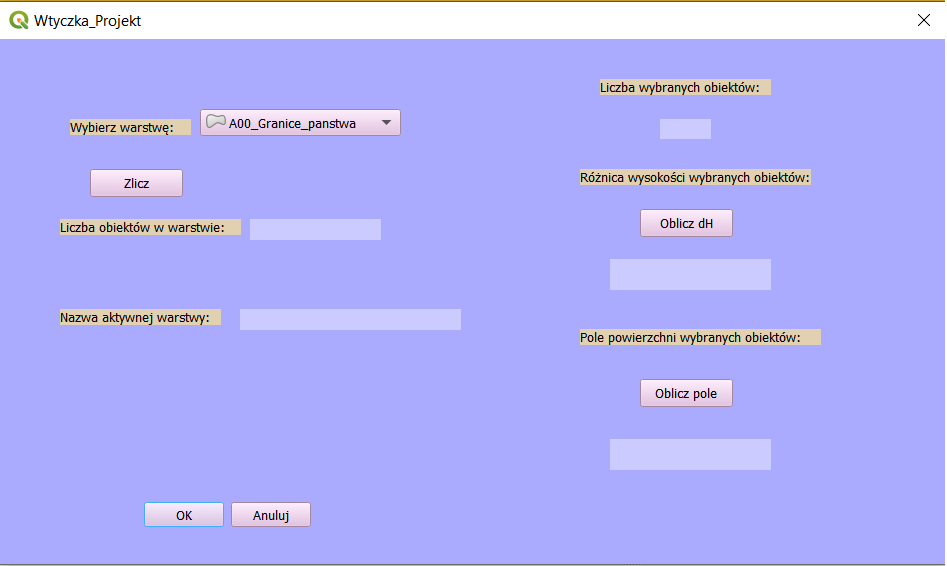
\includegraphics[width=1\textwidth]{wtyczunia.png}
	\end{figure}
		\subsection{Wybór opcji}
		Wtyczka umożliwia wybór zaimportowanych warstw w danym pliku. Poprzez kliknięcie przycisku $ Zlicz$ wyświetla się ilość obiektów znajdujących się w wybranej warstwie.\\
		Jeżeli chcemy obliczyć różnicę wysokości wybiera się obiekty punktowe danej warstwy a następnie klika się przycisk $Oblicz  dH$. Analogicznie postępuje się w przypadku obliczenia pola powierzchni. Należy wybierać odpowiednią ilość punktów. W przeciwnym razie będzie wyskakiwał odpowiedni komunikat informujący o występującym błędzie oraz co należy zrobić, aby obliczenia zostały przeprowadzone.
	\subsection{Przykład wykonanych obliczeń}
	\begin{figure}[H]
		\centering
		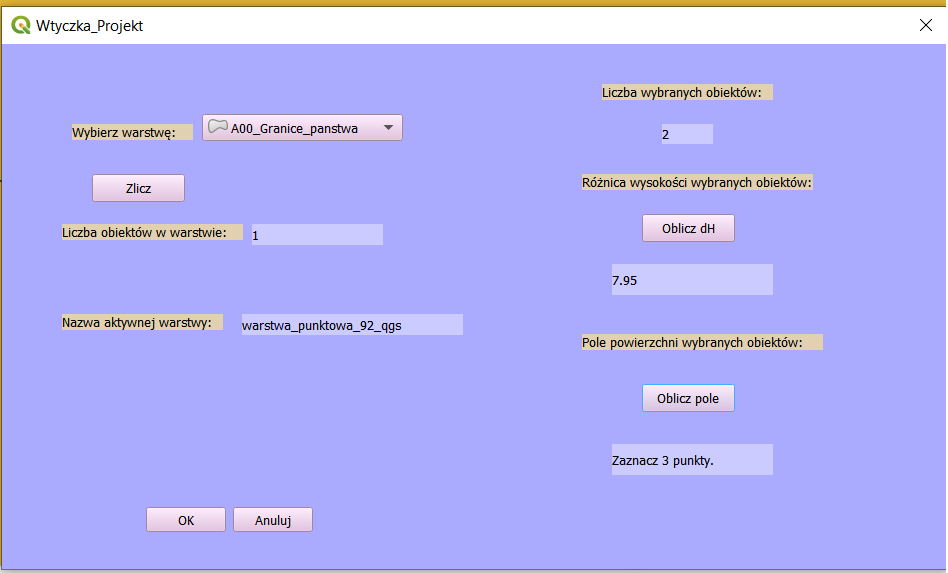
\includegraphics[width=1\textwidth]{dz.png}
		\end{figure}
	\begin{figure}[H]
		\centering
		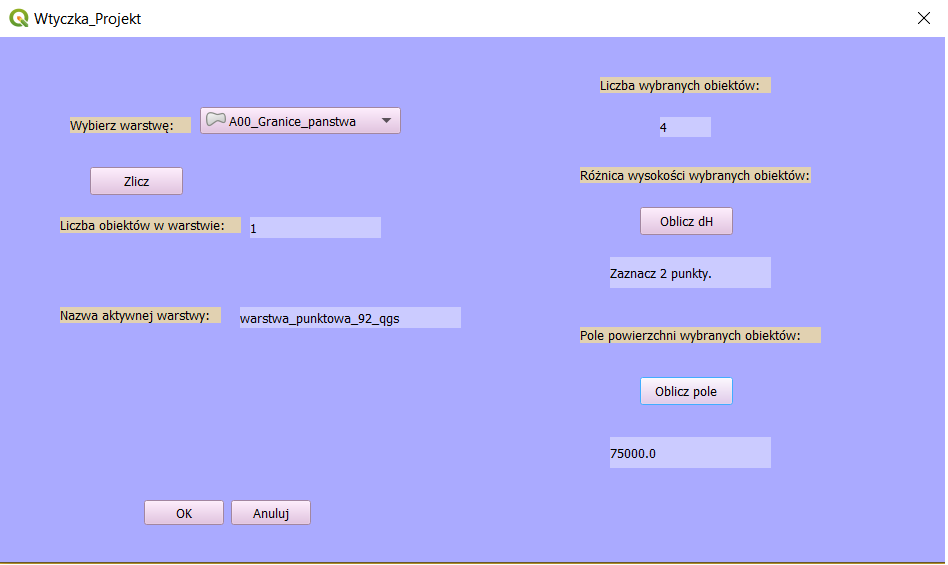
\includegraphics[width=1\textwidth]{dp.png}
	\end{figure}
\end{document}